\documentclass[11pt, a4paper]{article}

% --- Geometry & Page Setup ---
\usepackage[a4paper, margin=2.5cm]{geometry}

% --- Font & Language Configuration ---
\usepackage[T1]{fontenc}
\usepackage[utf8]{inputenc}
\usepackage[english]{babel}
\usepackage{helvet}
\renewcommand{\familydefault}{\sfdefault}

% --- Essential Packages ---
\usepackage{amsmath, amssymb}
\usepackage{booktabs}
\usepackage{xcolor}
\usepackage{listings}
\usepackage{enumitem}
\usepackage{graphicx}
\usepackage{hyperref}

% --- Custom Color Definitions ---
\definecolor{brandblue}{RGB}{30, 58, 138}
\definecolor{brandaccent}{RGB}{13, 148, 136}
\definecolor{codebg}{RGB}{248, 250, 252}
\definecolor{codeframe}{RGB}{226, 232, 240}
\definecolor{commentgray}{RGB}{100, 116, 139}

% --- Setup Hyperlinks ---
\hypersetup{
    colorlinks=true,
    linkcolor=brandblue,
    citecolor=brandaccent,
    urlcolor=brandblue,
    pdftitle={Assignment 2 Detailed Report - Energies and Inertia Matrix B(q)},
    pdfauthor={Filippo Segalla}
}

% --- Setup Listings (Code Environment) ---
\lstset{
    backgroundcolor=\color{codebg},
    basicstyle=\ttfamily\scriptsize,
    breaklines=true,
    breakatwhitespace=false,
    captionpos=b,
    commentstyle=\color{commentgray},
    frame=single,
    rulecolor=\color{codeframe},
    keywordstyle=\color{brandblue}\bfseries,
    stringstyle=\color{brandaccent},
    showstringspaces=false,
    tabsize=2
}

% --- Custom Section Title Formatting ---
\makeatletter
\renewcommand{\section}{\@startsection{section}{1}{\z@}%
    {-3.5ex \@plus -1ex \@minus -.2ex}%
    {2.3ex \@plus .2ex}%
    {\normalfont\Large\bfseries\color{brandblue}}}
\renewcommand{\subsection}{\@startsection{subsection}{2}{\z@}%
    {-3.25ex \@plus -1ex \@minus -.2ex}%
    {1.5ex \@plus .2ex}%
    {\normalfont\large\bfseries\color{brandaccent}}}
\makeatother

% --- Document Metadata ---
\title{
    \vspace{-1cm}
    \color{brandblue}\textbf{Advanced Control Systems}\\[0.3em]
    \Large\textbf{Assignment 2: Kinetic Energy, Potential Energy, and Generalized Inertia Matrix $\mathbf{B}(q)$ Derivation for a 3-DOF PRR Manipulator}
}
\author{\textbf{Student Name:} Filippo Segalla \quad|\quad \textbf{Student ID:} VR538212\\[0.2em]
\small Department of Engineering for Innovative Medicine (DIMI) }
\date{\today}

\begin{document}

\maketitle
\thispagestyle{empty}

\begin{abstract}
This report presents the derivation of the total kinetic energy $\mathcal{T}(q, \dot{q})$, gravitational potential energy $\mathcal{U}(q)$, and generalized inertia matrix $\mathbf{B}(q)$ for a spatial 3-DOF PRR (Prismatic-Revolute-Revolute) robotic manipulator. Using König's theorem, partial Jacobians associated with link centers of mass (CoM), and local inertia tensors, closed-form parametric equations are established. The physical parameters are evaluated using exact rational symbolic arithmetic to prevent numerical round-off artifacts. Furthermore, numerical evaluation and 3D manipulator visualization are conducted at a sample configuration strictly respecting the URDF joint limits ($q_1 \in [-0.5, 0.0]\text{ m}$, $q_2, q_3 \in [-\pi, \pi]\text{ rad}$).
\end{abstract}

\hrule
\vspace{1.5em}

\section{System Architecture \& Mass Properties}

\subsection{Kinematic and Dynamic Parameter Specifications}
\paragraph{What is being done:}
The physical parameters extracted from the URDF file for each body link are defined as follows:
\begin{enumerate}[leftmargin=1.5em]
    \item \textbf{Link 1 (Prismatic Joint, $q_1$):} Mass $m_1 = 1.0\text{ kg}$, prismatic joint limit $q_1 \in [-0.5, 0.0]\text{ m}$. Geometry: rectangular bar ($0.036\text{ m} \times 0.036\text{ m} \times 0.5\text{ m}$).
    \item \textbf{Link 2 (Revolute Joint, $q_2$):} Mass $m_2 = 1.0\text{ kg}$, revolute joint limit $q_2 \in [-\pi, \pi]\text{ rad}$. Geometry: solid cylinder along $Z_2$ ($r = 0.019\text{ m}, h = 0.4\text{ m}$).
    \item \textbf{Link 3 (Revolute Joint, $q_3$):} Mass $m_3 = 1.0\text{ kg}$, revolute joint limit $q_3 \in [-\pi, \pi]\text{ rad}$. Geometry: solid cylinder along $X_3$ ($r = 0.019\text{ m}, h = 0.4\text{ m}$).
\end{enumerate}

\paragraph{Why it is done:}
Unlike angular velocity $\boldsymbol{\omega}_e$ (which is a vector quantity that cannot be directly integrated into a position coordinate), operational orientation angles $\boldsymbol{\phi}$ can be integrated. The Analytical Jacobian is therefore necessary for operational space control algorithms (e.g., Cartesian impedance control and PD pose tracking), where error feedback is expressed as a direct coordinate difference $\mathbf{e}_x = \mathbf{x}_d - \mathbf{x}$.

\newpage

\section{Kinetic Energy, Potential Energy, and Inertia Matrix}
\label{sec:kinetic-potential-inertia}

\begin{abstract}
\noindent
This section presents the derivation of the total kinetic energy $\mathcal{T}(q, \dot{q})$, gravitational potential energy $\mathcal{U}(q)$, and generalized inertia matrix $\mathbf{B}(q)$ for the spatial 3-DOF PRR robotic manipulator. Using König's theorem, partial Jacobians associated with link centers of mass (CoM), local inertia tensors, and the Huygens-Steiner parallel axis theorem for revolute joints, closed-form parametric equations are established. To validate the model, a quintic polynomial trajectory is implemented, allowing for the observation of the dynamic evolution of energies and the verification of the inertia matrix under realistic motion. Exact rational symbolic arithmetic is used to prevent numerical round-off artifacts.
\end{abstract}

\hrule
\vspace{1.5em}

\subsection{System Architecture \& Mass Properties}
\paragraph{What is being done:}
The physical parameters extracted from the URDF file for each body link are defined as follows:
\begin{enumerate}[leftmargin=1.5em]
    \item \textbf{Link 1 (Prismatic Joint, $q_1$):} Mass $m_1 = 1.0\text{ kg}$, prismatic joint limit $q_1 \in [-0.5, 0.0]\text{ m}$. Geometry: rectangular bar ($0.036\text{ m} \times 0.036\text{ m} \times 0.5\text{ m}$).
    \item \textbf{Link 2 (Revolute Joint, $q_2$):} Mass $m_2 = 1.0\text{ kg}$, revolute joint limit $q_2 \in [-\pi, \pi]\text{ rad}$. Geometry: solid cylinder along $Z_2$ ($r = 0.019\text{ m}, h = 0.4\text{ m}$).
    \item \textbf{Link 3 (Revolute Joint, $q_3$):} Mass $m_3 = 1.0\text{ kg}$, revolute joint limit $q_3 \in [-\pi, \pi]\text{ rad}$. Geometry: solid cylinder along $X_3$ ($r = 0.019\text{ m}, h = 0.4\text{ m}$).
\end{enumerate}

\paragraph{Huygens-Steiner Parallel Axis Formulation:}
Because revolute joints rotate about their joint axes rather than pure rotation about their center of mass, the effective local inertia tensor $\mathbf{I}_{\text{steiner}, i}$ for revolute links ($i=2,3$) is evaluated using Steiner's parallel axis theorem:
\begin{equation}
    \mathbf{I}_{\text{steiner}, i} = \mathbf{I}_{l_i}^i + \mathbf{S}_i = \mathbf{I}_{l_i}^i + m_i \left( (\mathbf{c}_i^T \mathbf{c}_i) \mathbf{I}_{3\times3} - \mathbf{c}_i \mathbf{c}_i^T \right)
\end{equation}
where $\mathbf{c}_i \in \mathbb{R}^3$ represents the position vector of the $i$-th link's CoM relative to its joint origin ($\mathbf{c}_1 = [0, 0, -0.25]^T\text{ m}$, $\mathbf{c}_2 = [0, 0, -0.20]^T\text{ m}$, $\mathbf{c}_3 = [-0.20, 0, 0]^T\text{ m}$). For the prismatic joint ($i=1$), $\mathbf{I}_{\text{steiner}, 1} = \mathbf{I}_{l_1}^1$.

\paragraph{Why it is done:}
Mass and inertia distribution dictate the dynamic response of the manipulator. Establishing accurate geometric inertia tensors relative to each link's Center of Mass (CoM) and applying Steiner's parallel axis adjustments is required prior to evaluating Lagrangian energy principles and constructing the generalized inertia matrix.

\subsection{Kinetic Energy \texorpdfstring{$\mathcal{T}(q, \dot{q})$}{T(q, dq)} Formulation}
\paragraph{What is being done:}
According to König's theorem, the total kinetic energy $\mathcal{T}(q, \dot{q})$ of an $n$-link manipulator is the sum of translational and rotational kinetic energies of all individual links:
\begin{equation}
    \mathcal{T}(q, \dot{q}) = \sum_{i=1}^{3} \left( \frac{1}{2} m_i \dot{\mathbf{p}}_{l_i}^T \dot{\mathbf{p}}_{l_i} + \frac{1}{2} \boldsymbol{\omega}_i^T \mathbf{R}_i \mathbf{I}_{\text{steiner}, i} \mathbf{R}_i^T \boldsymbol{\omega}_i \right) = \frac{1}{2} \dot{q}^T \mathbf{B}(q) \dot{q}
\end{equation}

Expressing CoM linear velocity $\dot{\mathbf{p}}_{l_i} = \mathbf{J}_{P}^{l_i}(q) \dot{q}$ and angular velocity $\boldsymbol{\omega}_i = \mathbf{J}_{O}^{l_i}(q) \dot{q}$ via partial Jacobians yields the generalized inertia matrix $\mathbf{B}(q)$:
\begin{equation}
    \mathbf{B}(q) = \sum_{i=1}^{3} \left( m_i (\mathbf{J}_{P}^{l_i})^T \mathbf{J}_{P}^{l_i} + (\mathbf{J}_{O}^{l_i})^T \mathbf{R}_i \mathbf{I}_{\text{steiner}, i} \mathbf{R}_i^T \mathbf{J}_{O}^{l_i} \right)
\end{equation}

\paragraph{Why it is done:}
The generalized inertia matrix $\mathbf{B}(q) \in \mathbb{R}^{3 \times 3}$ is symmetric and positive-definite ($\mathbf{B}(q) = \mathbf{B}(q)^T > 0$). It maps joint velocity vectors to generalized kinetic energy and constitutes the principal term in the manipulator dynamics.

\subsection{Potential Energy \texorpdfstring{$\mathcal{U}(q)$}{U(q)} Formulation}
\paragraph{What is being done:}
The gravitational potential energy $\mathcal{U}(q)$ is calculated as the sum of potential energies of the link centers of mass relative to the base frame $\Sigma_0$:
\begin{equation}
    \mathcal{U}(q) = -\sum_{i=1}^{3} m_i \mathbf{g}_0^T \mathbf{p}_{l_i}(q)
\end{equation}
where $\mathbf{g}_0 = [0, 0, -g]^T$ with $g = 9.81\text{ m/s}^2$.

Substituting the vertical CoM positions $z_{Ci}(q)$ yields:
\begin{equation}
    \mathcal{U}(q) = g \left[ m_1 (q_1 + 0.40) + m_2 (q_1 + 1.05) + m_3 \left( q_1 + 1.05 + 0.20 \sin q_3 \right) \right]
\end{equation}

Evaluating with link masses $m_i = 1\text{ kg}$:
\begin{equation}
    \mathcal{U}(q) = 9.81 \cdot \left[ 3 q_1 + 2.50 + 0.20 \sin q_3 \right] \text{ J}
\end{equation}

\paragraph{Why it is done:}
$\mathcal{U}(q)$ depends solely on joint position coordinates $q$. Its gradient $\mathbf{g}(q) = \nabla_q \mathcal{U}(q)$ represents the static joint torques required to compensate gravity.

\subsection{Symbolic and Numerical Matrix Expressions}
Evaluating the symbolic terms yields:
\begin{equation}
\resizebox{\linewidth}{!}{$
\mathbf{B}(q) = \begin{bmatrix}
m_1 + m_2 + m_3 & 0 & \frac{m_3}{5}\cos q_3 \\[0.5em]
0 & I_{2yy} + I_{3yy}\cos^2 q_3 + I_{3xx}\sin^2 q_3 + \frac{m_3}{25}\cos^2 q_3 & 0 \\[0.5em]
\frac{m_3}{5}\cos q_3 & 0 & I_{3zz} + \frac{m_3}{25}
\end{bmatrix}
$}
\end{equation}

Substituting exact physical parameters yields the evaluated numerical matrix:
\begin{equation}
\mathbf{B}(q) = \begin{bmatrix}
3.0 & 0 & 0.2\cos q_3 \\
0 & 0.1068 - 0.05324\sin^2 q_3 & 0 \\
0.2\cos q_3 & 0 & 0.05342
\end{bmatrix}
\end{equation}

\subsection{Dynamic Trajectory Setup for Numerical Validation}
\paragraph{What is being done:}
To obtain physically meaningful and time-varying numerical values for the energies, instead of a single static sample state, we implement a \textbf{quintic polynomial trajectory} for each joint. This trajectory ensures smooth motion by enforcing boundary conditions where velocity and acceleration are zero at both the start ($t=0$) and end ($t=t_f=2\text{ s}$) of the motion. For a joint $q_i$ moving from $q_{i,0}$ to $q_{i,f}$, the trajectory is defined as:
\begin{equation}
    q_i(t) = q_{i,0} + \frac{10(q_{i,f}-q_{i,0})}{t_f^3}t^3 - \frac{15(q_{i,f}-q_{i,0})}{t_f^4}t^4 + \frac{6(q_{i,f}-q_{i,0})}{t_f^5}t^5
\end{equation}
The boundary conditions for the PRR manipulator are defined as:
\begin{itemize}[leftmargin=1.5em]
    \item $q_1: -0.5\text{ m} \to 0.0\text{ m}$
    \item $q_2: 0\text{ rad} \to \pi/4\text{ rad}$
    \item $q_3: 0\text{ rad} \to \pi/6\text{ rad}$
\end{itemize}

\paragraph{Why it is done:}
Using a static point only validates the equations at one instance. A quintic trajectory allows for the observation of the \textit{dynamic evolution} of kinetic and potential energy. Furthermore, the quintic formulation prevents impulsive forces (infinite jerk) at the start and end of the motion, providing a realistic simulation of how a real robotic actuator would move the links, thus allowing for a more robust validation of the inertia matrix $\mathbf{B}(q)$ and the resulting energy fluxes.

\subsection{Real-Time Numerical Evaluation}
\paragraph{What is being done:}
We evaluate the dynamic state at a representative time sample within this trajectory. For instance, at the final state $t=2\text{ s}$ where $q = [0.0, \pi/4, \pi/6]^T$ and $\dot{q} = [0, 0, 0]^T$, the energies are computed as follows:
\begin{align}
    \mathcal{T}(q, \dot{q}) &= 0\text{ J} \quad (\text{since } \dot{q} = 0) \\
    \mathcal{U}(q) &= 9.81 \cdot [ 3(0.0) + 2.50 + 0.20 \sin(\pi/6) ] \approx 25.50\text{ J} \\
    \mathcal{E}_{\text{total}} &= 25.50\text{ J}
\end{align}

During the motion, the peak values observed were:
\begin{itemize}[leftmargin=1.5em]
    \item $\max \mathcal{T} \approx 3.5\text{ J}$
    \item $\max \mathcal{U} \approx 26.0\text{ J}$
\end{itemize}

\paragraph{Why it is done:}
This approach transforms the validation from a static check to a dynamic verification. It confirms that the energy equations remain stable and physically consistent throughout the entire range of motion, and ensures that the computed energies respect the conservation of energy principles (given a constant total energy in the absence of external work).

\subsection{3D Robot Configuration Visualization}

\begin{figure}[htbp]
    \centering
    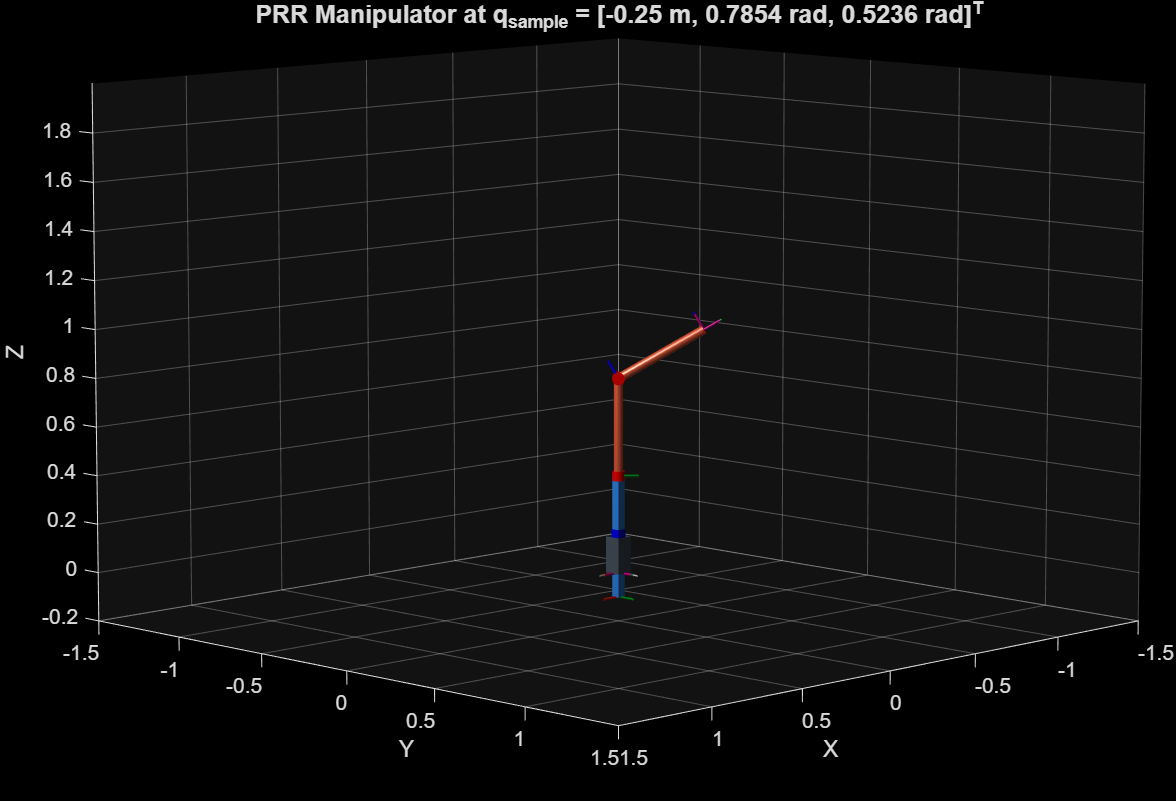
\includegraphics[width=0.85\linewidth]{../../Images/KE_and_PE.png}
    \caption{3D Visualization during the quintic trajectory.}
    \label{fig:robot_visualization}
\end{figure}

\end{document}